\documentclass[
	11pt,
	t,
]{beamer}

\setbeamertemplate{caption}[numbered]

\graphicspath{{images/}{./}}

\usepackage{tikz}
\usetikzlibrary{positioning}

\usepackage{booktabs}
\usetheme{Madrid}
\usecolortheme{lily}
\usefonttheme{default}
\usepackage{palatino}

\usepackage[default]{opensans}
\useinnertheme{circles}

\title[Computer Science and College]{Computer Science and College}

\author[Sachin Iyer]{Sachin Iyer}

\institute[NYU]{New York University \\ \smallskip \textit{sachiniyer@nyu.edu}}

\date[\today]{\today}

%----------------------------------------------------------------------------------------

\begin{document}

\begin{frame}
	\titlepage
\end{frame}

\begin{frame}
	\frametitle{Agenda}
	\tableofcontents[pausesections]
\end{frame}

\section{Demonstration}

\begin{frame}
	\frametitle{Demonstration}
	\href{https://school-demo.sachiniyer.com}{https://school-demo.sachiniyer.com}
	\bigskip
	\begin{figure}
	  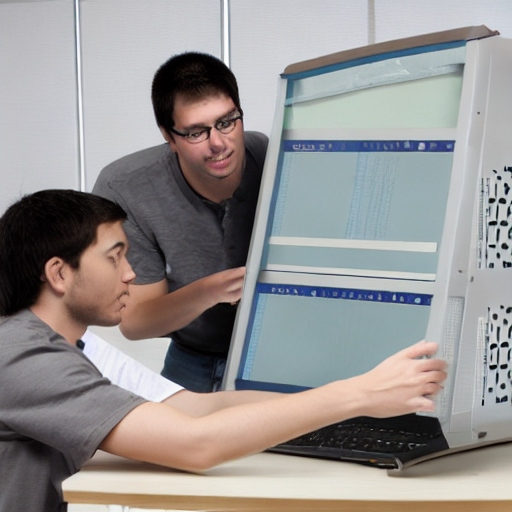
\includegraphics[scale=0.17]{1.jpg}
	  \caption{People looking into a computer screen}
	\end{figure}
\end{frame}


\section{Explanation}
\subsection{Actors involved}

\begin{frame}
	\frametitle{Actors involved}
	\begin{columns}
	  \begin{column}{0.7\textwidth}
		\begin{itemize}
		  \item Your device (phone, computer, tablet) \\
		  \item My computers with public internet access \\
		  \item My laptop \\
		  \item The LED screen \\
		\end{itemize}
	  \end{column}
	  \begin{column}{0.3\textwidth}
		\begin{center}
		  \begin{figure}
			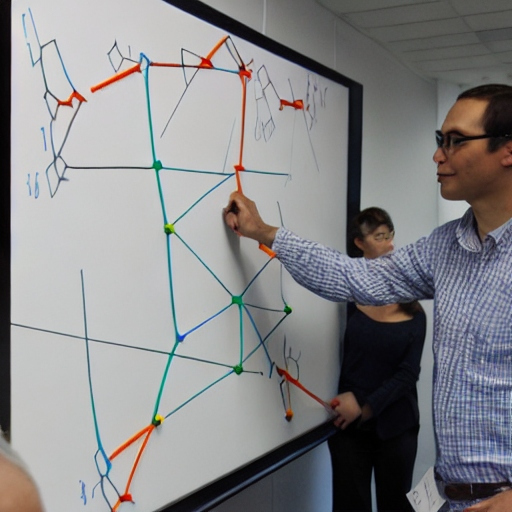
\includegraphics[scale=0.17]{2.jpg}
			\caption{A teacher explaining a concept}
		  \end{figure}
		\end{center}
	  \end{column}
	\end{columns}
\end{frame}

\subsection{Graph of Information}
\begin{frame}[fragile]
  \frametitle{Graph of Information}
  \bigskip \centering

    \begin{tikzpicture}
  \matrix [column sep=20mm, row sep=4mm] {
    &  \node (a) [draw, shape=circle] {My computers}; & \\
    \node (c) [draw, shape=circle] {Your device}; & &
    \node (e) [draw, shape=circle] {My computer}; \\
    & & \node (i) [draw, shape=circle] {LED display}; \\
  };
    \draw[->, very thick] (c) -- (a);
    \draw[->, very thick] (a) -- (e);
    \draw[->, very thick] (e) -- (i);
  \end{tikzpicture}
\end{frame}

\section{College}

\begin{frame}
	\frametitle{College}
	\begin{columns}
	  \begin{column}{0.7\textwidth}
		\begin{itemize}
		  \item Learn how to make what I made \\
		  \item Meet other cool smart people \\
		  \item Have fun learning subject you want to learn \\
		  \item Gaining skills to do cool things the rest of your life \\
		\end{itemize}
	  \end{column}
	  \begin{column}{0.3\textwidth}
		\begin{center}
		  \begin{figure}
			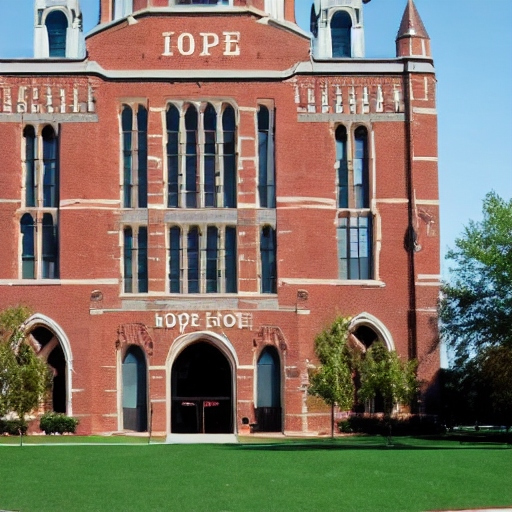
\includegraphics[scale=0.17]{3.jpg}
			\caption{A image of a college building}
		  \end{figure}
		\end{center}
	  \end{column}
	\end{columns}
\end{frame}

\section{Easter Egg}

\begin{frame}
	\frametitle{Easter Egg}
	All the images were created with Artificial Intelligence - a computer created them (\href{DeepAI}{https://deepai.org})
	\bigskip
	\begin{figure}
	  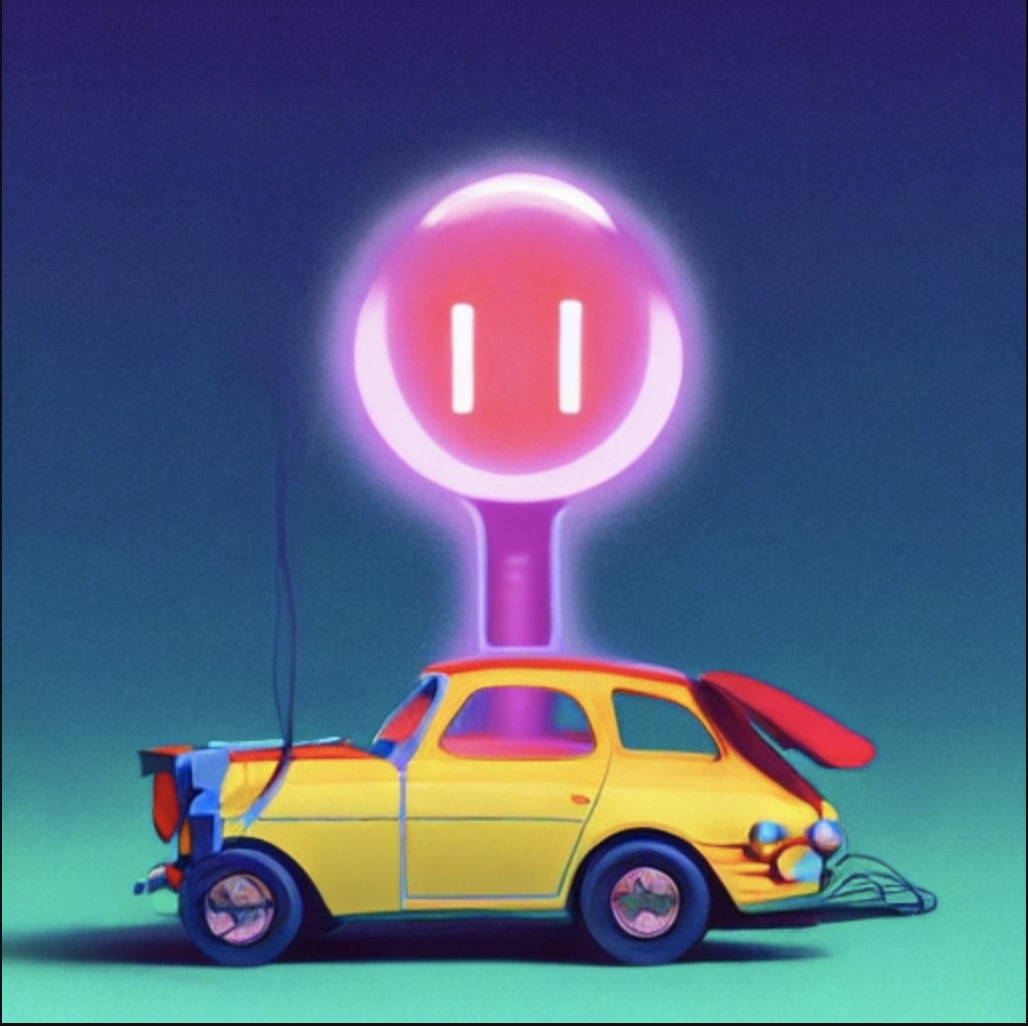
\includegraphics[scale=0.3]{4.jpg}
	  \caption{A futuristic car}
	\end{figure}
\end{frame}


\end{document}
